\chapter{Graph-Datenbanken - Grundlegende technologische Aspekte}
%\section{Einführung}
\section{Modell}
\subsection{Graph}
%@ToDo Motivation warum erklären wir Graphen?[Jenny]
%Ein Graph G besteht aus einer nichtleeren Menge an Knoten V und Kanten E.
Graphen eignen sich um Probleme zu abstrahieren oder zu modellieren.
Ein Graph ist mathematisch folgendermaßen definiert:
\begin{definition}
	Ein $\text{Graph} G=(V,E,\gamma)$ ist ein Tripel bestehend aus:
	\begin{itemize}
		\item $V$, einer nicht leeren Menge von Knoten(vertices)
		\item $E$, einer Menge von Kanten (edges) und
		\item $\gamma$ , einer Inzidenzabbildung (incidence relation), mit\\
		$\gamma : E \longrightarrow \{X | X \subseteq V, 1 \leq |X| \leq 2\}$
	\end{itemize}

	Ein Knoten $a \in V$ und eine Kante $e \in E$ heißen inzident (incident)
	genau dann wenn $a$ entweder Anfangs- oder Endecke von $e$ ist. Es gilt $a \in \gamma(e)$.
	Zwei Knoten $a,b \in V$ heißen adjazent(adjacent) genau dann wenn es eine Kante $e$ gibt die zu $a$ und $b$ inzident ist.
	Es gilt	$\exists e \in E: \gamma(e)=\{a,b\}$.\footnote{\cite[Seite 21]{pbeck01}} \\

\end{definition}
Die Kanten stellen die Beziehung zwischen den einzelnen Knoten her.
In einem klassischen Graphen kann eine Kante immer nur jeweils zwei Knoten miteinander verbinden.
Graphen können gerichtet oder ungerichtet sein. Gerichtete Graphen zeichnen sich dardurch aus, dass die Kanten eine zugewiesen Richtung besitzen.
Um die Beziehung zwischen zwei Knoten genauer zu definieren lassen sich die Kanten gewichten.
In diesem Fall werden den Kannten in der Regel nummerische Werte zugeordnet und man bezeichnet diese Graphen als Gewichtete Graphen.

%http://page.math.tu-berlin.de/~felsner/Lehre/GrTh05/Graphentheorie.pdf
Hat eine Kante als Start- und Endknoten den selben Knoten, verbindet also den Knoten mit sich selber, spricht man von einer Schlinge.
Liegen zwischen zwei Knoten eines Graphen mehr als eine Kante, nennt man diese Multikante.
Schlingen und Multikanten dürfen in einem klassischen Graphen nicht auftauchen.\cite{}

Werden Kanten und Knoten eines Graphs vertauscht entsteht der Kantengraph bzw. Line-Graph des jeweiligen Graphen L(G).
Zwei Graphen können isomorph sein.

Der Grad eines eines Knoten bezeichnet die Anzahl der inzidenten Kanten des Knoten. Dabei werden Schleifen doppelt gezählt.\footnote{Vgl. \cite[Seite 13]{rahm2017}}

\subsection{Reguläre Graphen}
%@ToDo Bilder einfügen
Bei Reguläre Graphen haben alle Knoten den selben Knotengrad.
Als Knotengrad wir die Anzahl direkter Nachbarn, also alle Knoten die über eine Kante direkt mit dem betrachteten Knoten verbunden sind, bezeichnet.\cite{felsner2012geometric}
\begin{center}
	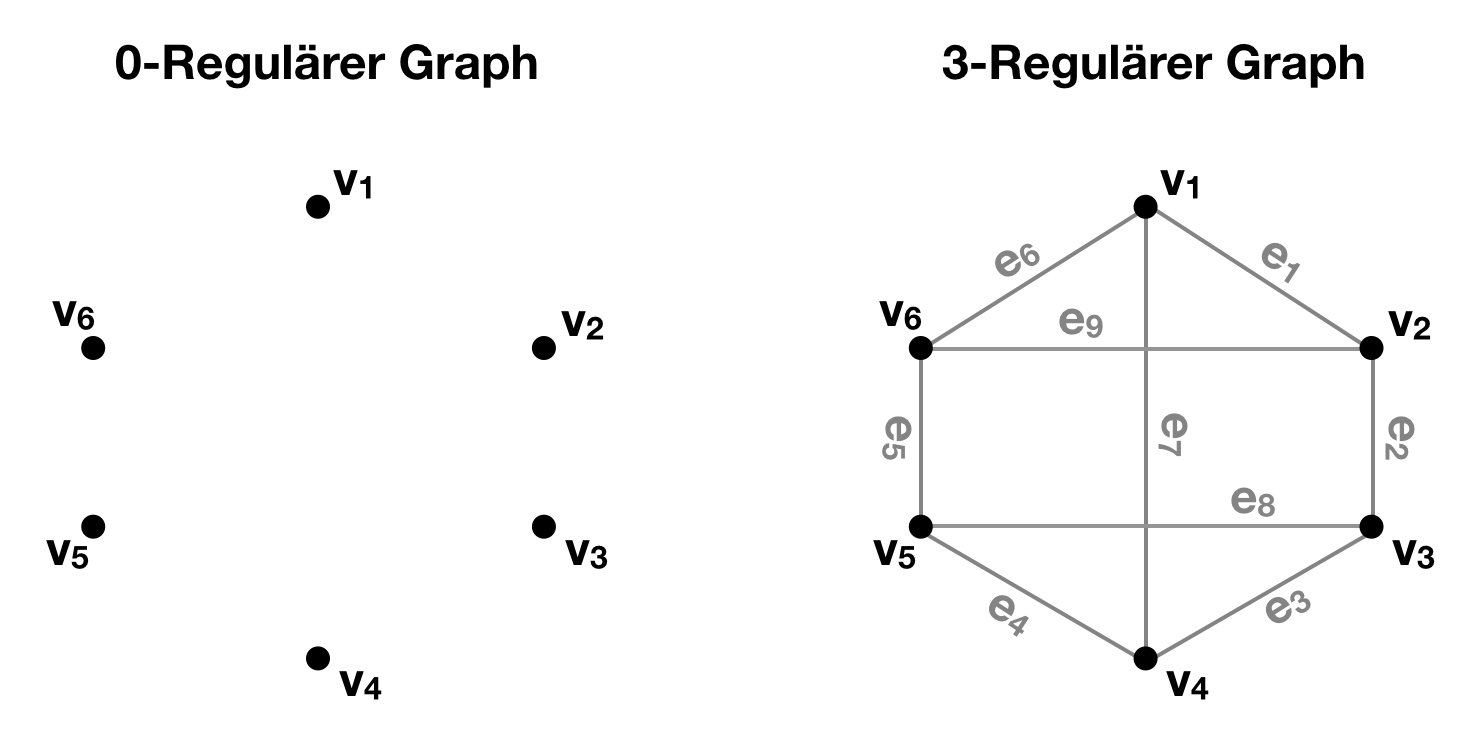
\includegraphics[scale = 0.5]{./images/Regulaerer_graph.png}
\end{center}
\subsection{Planare Graphen}
%@ToDo Bilder einfügen
Planare Graphen lassen sich in der Ebene ohne Überschneidung der Kanten zeichnen.\cite{Theobald2016}
\begin{center}
	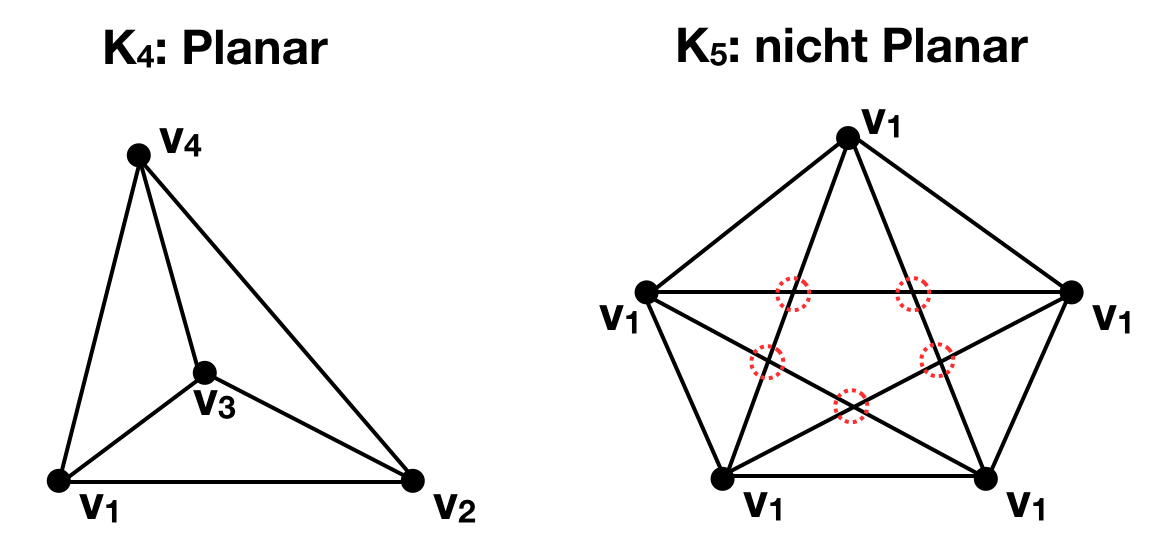
\includegraphics[scale = 0.5]{./images/planarer_graph.png}
\end{center}
\subsection{Property Graphen}
%@ToDo Bilder einfügen
Property Graphen zeichnen sich durch ihre den Kanten und Knoten zugewiesenen Eigenschaften aus.
\subsection{k-Partite Graphen}
%@ToDo Bilder einfügen
Die Knoten können in k Partitionen unterteilt werden, sodass die Knoten in einer Gruppe keine direkten Nachbarn sind.
\begin{center}
	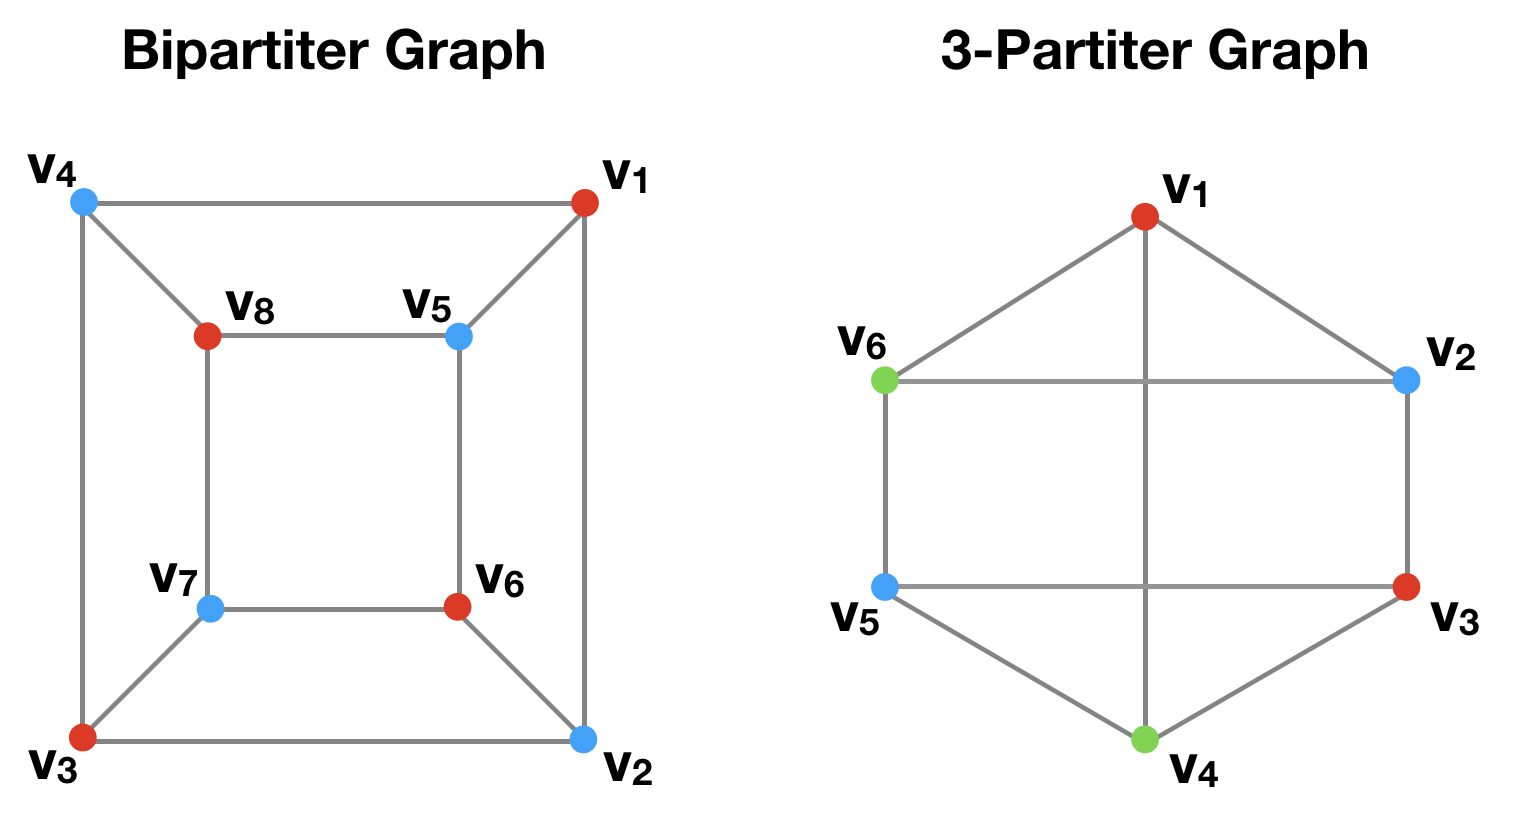
\includegraphics[scale = 0.4]{./images/k_partiter_graph.png}
\end{center}
\subsection{Hypegraphen}
Hypergraphen haben die Eigenschaft, dass Kanten im Gegensatz zu klassischen Graphen mehr als zwei Knoten miteinander verbinden können.
\\Mathematisch ist ein Hypergraph ist folgendermaßen definiert:
\begin{definition}
	Let $X=\{v_{1}, v_{2},...,v_{n}\}$ be a finite set,
	and let $E=\{e_{1},e_{2},...,e_{m}\}$ be a family of subsets of $X$ such that
	\[e_{i} \neq \varnothing (i=1,2,...,m) \\
	\cup_{i=1}^{m}e_{i}=X.
	\]
	The pair $H=(X,E)$ is called a hypergraph with vertex set $X$
	and hyperedge set $E$. The elements $v_{1}, v_{2},...,v_{n}$ of $X$ are vertices
	of hypergraph $H$, and the sets $e_{1}, e_{2},...,e_{m}$ are hyperedges of hypergraph $H$.\footnote{Vgl. \cite[Seite 2]{zhang2018hypergraph}}
\end{definition}
Das folgende Bild zeigt einen Hypergraphen:
\begin{center}
	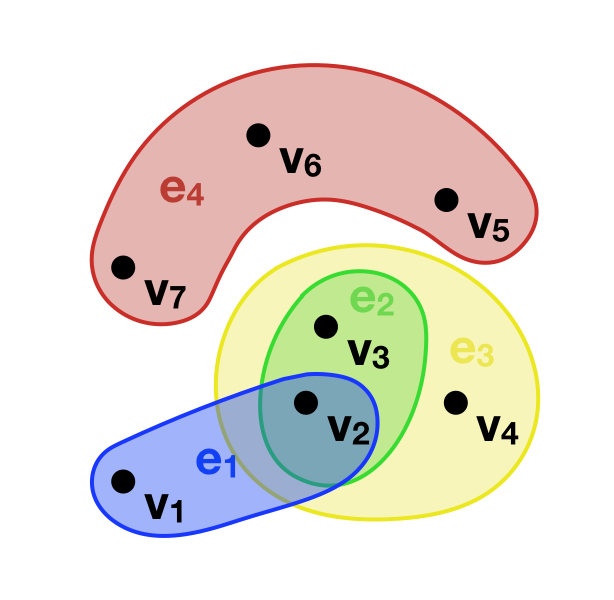
\includegraphics[scale = 0.5]{./images/Hypergraph2.png}
\end{center}
Im Vergleich zum normale Graphen können die Kanten eines Hypergraphen eine beliebige Kardinalität haben (siehe Definition Definition Graph Kapitel 1.2.1) . Beim normalen Graphen können die Kanten nur die Kardinalität $1 \leq |X| \leq 2$
haben. Die Hyperedges in einem Hypergraphen sind somit eine beliebige Menge von Knoten. In einem normale Graphen sind die Kanten, eine in einem Intervall festgelegte Menge von Knoten:
    \[X = \{v_{1}, v_{2}, v_{3}, v_{4}, v_{5}, v_{6}, v_{7}\} \text{ Knoten}\]
    \[E=\{e_{1}, e_{2}, e_{3}, e_{4}\} \text{ Kanten}\]
    \[E=\{e_{1}, e_{2}, e_{3}, e_{4}\} = \{\{v_{1}, v_{2}, v_{3}\}, \{v_{2}, v_{3}\}, \{v_{3}, v_{5}, v_{6}\}, \{v_{4}\}\} \]
\subsection{Multimodale Graphen}